\chapter{Performance}

\section{Learning}
During our learning sessions we did try different values for our network, but
didn't try different topologies after doing the initial tests. We landed upon
having a topology with a single hidden layer consisting of 10 perceptrons. The
learning algorithm with back propagation was then run a 100.000 times on the
entire testing dataset to reduce the errors. After a couple of initial tests at
30.000 runs, there was still some perceptrons that didn't converge fully but had
an offset from the target value of 0.01.

This was by far the worst offset from target value, but mostly because we had
set the threshold at 0.004.

There are also some other choices we made which may have resulted in a worse
time performance since we are allways doing weight updates, even when the
perceptron is within its target output.  But we have not made these tests to
know for sure.

Below we have recorded some statistics of how long it took to learn and run the
different set, to illustrate the differences. As you can see the last run had a
maximum offset from target of 0.0049, which is more than tolerable and adequate
for testing.  The calculated error values for the perceptron is considered equal
to zero since they are so low.

\begin{longtable}{ p{0.15\textwidth} p{0.1\textwidth} p{0.15\textwidth} 
									 p{0.075\textwidth} c r }
\textbf{Data set} & \textbf{Epochs}		& \textbf{Time} 			& & 
									  \textbf{Error}		& \textbf{Off Targ} \\\hline 
1-10	& 100.000 & 00:24:54.194	& MAX 	& 0.0000	& 0.0049 	\\
			& 				& 							& MIN 	& 0.0000	& -0.0038	\\
			& 				& 							& AVG 	& 0.0000	& -0.0001	\\
11-20	& 100.000 & 00:25:15.142	& MAX 	& 0.0000	& 0.0045	\\
			& 				& 							& MIN 	& 0.0000	& -0.0035	\\
			& 				& 							& AVG 	& 0.0000	& -0.0001	\\
Mixed & 100.000 & 00:23:35.945	& MAX 	& 0.0000	& 0.0046	\\
dataset	& 			& 							& MIN 	& 0.0000	& -0.0040	\\
				& 			& 							& AVG 	& 0.0000	& -0.0001	\\
\end{longtable}

\section{Testing}
For our testing we ran four test using our final 2 sets of network training
weights.  We ran, as show in the next chapter, the four tests: learn data set
1-10 and test both data set 1-10 and 11-20 against the resulting network. Learn
data set 11-20 and test both data set 1-10 and 11-20 against the resulting
network.  The resulting information is then feed into a spreadsheet program as a
CSV file where we do some quick calculations and editing before exporting them
to the report format shown in the result chapter.

The summary of the data presented in the next chapter are the averaged values of
the the 10 data sets it is being ran through.  This means that the represented
values in the tables are the average of 10 runs per character.  This means that
some of the data sets will have a different value, than the rest.

A short summary of the data is that we have a good network that can identify
very well the data set it was trained with. It performs adequately against the
opposite dataset in accordance to which we trained with. When testing the
opposite data set we receive a good amount of errors, but it is mostly able to
identify the correct characters with a mid-range certainty.

Overall performance of the network is relatively good. It should be pointed out
that we could have implemented more tests and tested different topologies, but
due to programming errors and wasted time it was left undone. But the program is
very modular and can easily perform testing.

\subsection{Data set review}
We have provided two types of tables, the first set of tables(\ref{tab:dtaA},
\ref{tab:dtaB}, \ref{tab:dtaC}, \ref{tab:dtaD}, \ref{tab:dtabiAVG}), are the
displaying the averaged percentage for how much the data set is reckognised as
that particular character.  The other type of table(\ref{tab:dtaA_ID},
\ref{tab:dtaB_ID}, \ref{tab:dtaC_ID}, \ref{tab:dtaD_ID}, \ref{tab:dtabiID}),
is displaying out of the number of test it was reckognised as that specific
character with a rate equal to or more tha 50\%.

As shown in all of the tables for learning and testing the ANN with the same
data we are receiveing full score for those data set, tables
\ref{tab:dtaA}/\ref{tab:dtaA_ID} and \ref{tab:dtaD}/\ref{tab:dtaD_ID}.  This is
because we test against the same data sets which we've been training on.

One of the features to note from this is the diagonal that is being displayed in
the matrix of values.  It shows that the characters are, in fact, being
interpreted as the correct characters by the ANN.

So on the opposite side where we test against the data sets which we haven't
trained for the reckognition rate drops severly, but it still shows that most of
the times they are reckognised correctly.  This is shown in tables 
\ref{tab:dtaB}/\ref{tab:dtaB_ID} and \ref{tab:dtaC}/\ref{tab:dtaC_ID}, and even
though the values are much more spread out we still can see the trend that the
diagonal as in the said above is still appearing. Though, much weaker.

As our final test we took a mixed data set(1, 3, 5, 7, 9, 11, 13, 15, 17, 19) as
our training set since this provides the best blend of values from the dataset.
As opposed to the segragated dataset used previously.  We trained the ANN
100.000 on this data and ran it against the enitre dataset from 1-20.  The
resulting values are shown in table \ref{tab:dtabiAVG} and \ref{tab:dtabiID}.
In table \ref{tab:dtabiAVG}, we've displayed the average of how much it
reckognises a character as the different characters. In table \ref{tab:dtabiID}
we have noted how many times the dataset is reckognised as the actual characters
with a percentage of more that 50\%.


\subsection{Conclusion}
The reason for our wery low value when running the oposite data set is because
these two parts are very different for most of the values.  It is also because
of our generalisation function which generalizes the 30x30 pixel image into
10x10 pixel values. Thes 100 pixel values from 0 to 255 is then also generalized
even further by declaring that any value beyond or equal to 200 is equal to 0
and anythinf below this value is equal to 1.  This creates a very harsh
generalisation of the images and will impact the images vastly.

However when we test against the same data set we receive perfect scores which
is very good, but easy since it is the same data sets.

When we trained the ANN against a mixed data set we received better results when
testing it later on. We tested it on the entire dataset which yields good
results where it both identifies the correct character and has good detection
rate.  However the table provided is slightly biased since half of the values
it is tested on is the same as the training set, but it shows that it is
detecting the characters relatively reliably.

As stated above, some of the data sets is not specially similar in the way they
are constructed as depicted below.  Especially the data sets for ''A'' can be split
into two sets which has very distinct looks and thus will not identify eachother
well if trained exlusively with one of them.  The ''Z'' set doesn't split as
easily into different data sets and is thus much easier to train and identify
later on. 

\begin{figure}[h]
\centering
\begin{minipage}{0.04\textwidth}
	
\includegraphics[width=\textwidth]{../pics/A1}
\end{minipage}
\begin{minipage}{0.04\textwidth}
	
\includegraphics[width=\textwidth]{../pics/A2}
\end{minipage}
\begin{minipage}{0.04\textwidth}
	
\includegraphics[width=\textwidth]{../pics/A3}
\end{minipage}
\begin{minipage}{0.04\textwidth}
	
\includegraphics[width=\textwidth]{../pics/A4}
\end{minipage}
\begin{minipage}{0.04\textwidth}
	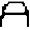
\includegraphics[width=\textwidth]{../pics/A5}
\end{minipage}
\begin{minipage}{0.04\textwidth}
	
\includegraphics[width=\textwidth]{../pics/A6}
\end{minipage}
\begin{minipage}{0.04\textwidth}
	
\includegraphics[width=\textwidth]{../pics/A7}
\end{minipage}
\begin{minipage}{0.04\textwidth}
	
\includegraphics[width=\textwidth]{../pics/A8}
\end{minipage}
\begin{minipage}{0.04\textwidth}
	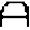
\includegraphics[width=\textwidth]{../pics/A9}
\end{minipage}
\begin{minipage}{0.04\textwidth}
	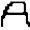
\includegraphics[width=\textwidth]{../pics/A10}
\end{minipage}
\begin{minipage}{0.04\textwidth}
	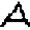
\includegraphics[width=\textwidth]{../pics/A11}
\end{minipage}
\begin{minipage}{0.04\textwidth}
	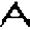
\includegraphics[width=\textwidth]{../pics/A12}
\end{minipage}
\begin{minipage}{0.04\textwidth}
	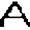
\includegraphics[width=\textwidth]{../pics/A13}
\end{minipage}
\begin{minipage}{0.04\textwidth}
	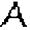
\includegraphics[width=\textwidth]{../pics/A14}
\end{minipage}
\begin{minipage}{0.04\textwidth}
	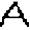
\includegraphics[width=\textwidth]{../pics/A15}
\end{minipage}
\begin{minipage}{0.04\textwidth}
	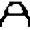
\includegraphics[width=\textwidth]{../pics/A16}
\end{minipage}
\begin{minipage}{0.04\textwidth}
	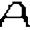
\includegraphics[width=\textwidth]{../pics/A17}
\end{minipage}
\begin{minipage}{0.04\textwidth}
	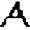
\includegraphics[width=\textwidth]{../pics/A18}
\end{minipage}
\begin{minipage}{0.04\textwidth}
	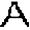
\includegraphics[width=\textwidth]{../pics/A19}
\end{minipage}
\begin{minipage}{0.04\textwidth}
	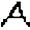
\includegraphics[width=\textwidth]{../pics/A20}
\end{minipage}

\begin{minipage}{0.04\textwidth}
	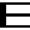
\includegraphics[width=\textwidth]{../pics/E1}
\end{minipage}
\begin{minipage}{0.04\textwidth}
	
\includegraphics[width=\textwidth]{../pics/E2}
\end{minipage}
\begin{minipage}{0.04\textwidth}
	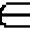
\includegraphics[width=\textwidth]{../pics/E3}
\end{minipage}
\begin{minipage}{0.04\textwidth}
	
\includegraphics[width=\textwidth]{../pics/E4}
\end{minipage}
\begin{minipage}{0.04\textwidth}
	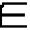
\includegraphics[width=\textwidth]{../pics/E5}
\end{minipage}
\begin{minipage}{0.04\textwidth}
	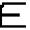
\includegraphics[width=\textwidth]{../pics/E6}
\end{minipage}
\begin{minipage}{0.04\textwidth}
	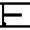
\includegraphics[width=\textwidth]{../pics/E7}
\end{minipage}
\begin{minipage}{0.04\textwidth}
	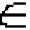
\includegraphics[width=\textwidth]{../pics/E8}
\end{minipage}
\begin{minipage}{0.04\textwidth}
	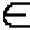
\includegraphics[width=\textwidth]{../pics/E9}
\end{minipage}
\begin{minipage}{0.04\textwidth}
	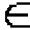
\includegraphics[width=\textwidth]{../pics/E10}
\end{minipage}
\begin{minipage}{0.04\textwidth}
	
\includegraphics[width=\textwidth]{../pics/E11}
\end{minipage}
\begin{minipage}{0.04\textwidth}
	
\includegraphics[width=\textwidth]{../pics/E12}
\end{minipage}
\begin{minipage}{0.04\textwidth}
	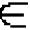
\includegraphics[width=\textwidth]{../pics/E13}
\end{minipage}
\begin{minipage}{0.04\textwidth}
	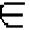
\includegraphics[width=\textwidth]{../pics/E14}
\end{minipage}
\begin{minipage}{0.04\textwidth}
	
\includegraphics[width=\textwidth]{../pics/E15}
\end{minipage}
\begin{minipage}{0.04\textwidth}
	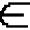
\includegraphics[width=\textwidth]{../pics/E16}
\end{minipage}
\begin{minipage}{0.04\textwidth}
	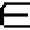
\includegraphics[width=\textwidth]{../pics/E17}
\end{minipage}
\begin{minipage}{0.04\textwidth}
	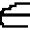
\includegraphics[width=\textwidth]{../pics/E18}
\end{minipage}
\begin{minipage}{0.04\textwidth}
	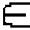
\includegraphics[width=\textwidth]{../pics/E19}
\end{minipage}
\begin{minipage}{0.04\textwidth}
	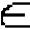
\includegraphics[width=\textwidth]{../pics/E20}
\end{minipage}

\begin{minipage}{0.04\textwidth}
	
\includegraphics[width=\textwidth]{../pics/S1}
\end{minipage}
\begin{minipage}{0.04\textwidth}
	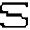
\includegraphics[width=\textwidth]{../pics/S2}
\end{minipage}
\begin{minipage}{0.04\textwidth}
	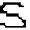
\includegraphics[width=\textwidth]{../pics/S3}
\end{minipage}
\begin{minipage}{0.04\textwidth}
	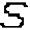
\includegraphics[width=\textwidth]{../pics/S4}
\end{minipage}
\begin{minipage}{0.04\textwidth}
	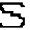
\includegraphics[width=\textwidth]{../pics/S5}
\end{minipage}
\begin{minipage}{0.04\textwidth}
	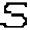
\includegraphics[width=\textwidth]{../pics/S6}
\end{minipage}
\begin{minipage}{0.04\textwidth}
	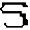
\includegraphics[width=\textwidth]{../pics/S7}
\end{minipage}
\begin{minipage}{0.04\textwidth}
	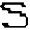
\includegraphics[width=\textwidth]{../pics/S8}
\end{minipage}
\begin{minipage}{0.04\textwidth}
	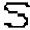
\includegraphics[width=\textwidth]{../pics/S9}
\end{minipage}
\begin{minipage}{0.04\textwidth}
	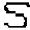
\includegraphics[width=\textwidth]{../pics/S10}
\end{minipage}
\begin{minipage}{0.04\textwidth}
	\includegraphics[width=\textwidth]{../pics/S11}
\end{minipage}
\begin{minipage}{0.04\textwidth}
	\includegraphics[width=\textwidth]{../pics/S12}
\end{minipage}
\begin{minipage}{0.04\textwidth}
	\includegraphics[width=\textwidth]{../pics/S13}
\end{minipage}
\begin{minipage}{0.04\textwidth}
	\includegraphics[width=\textwidth]{../pics/S14}
\end{minipage}
\begin{minipage}{0.04\textwidth}
	\includegraphics[width=\textwidth]{../pics/S15}
\end{minipage}
\begin{minipage}{0.04\textwidth}
	\includegraphics[width=\textwidth]{../pics/S16}
\end{minipage}
\begin{minipage}{0.04\textwidth}
	\includegraphics[width=\textwidth]{../pics/S17}
\end{minipage}
\begin{minipage}{0.04\textwidth}
	\includegraphics[width=\textwidth]{../pics/S18}
\end{minipage}
\begin{minipage}{0.04\textwidth}
	\includegraphics[width=\textwidth]{../pics/S19}
\end{minipage}
\begin{minipage}{0.04\textwidth}
	\includegraphics[width=\textwidth]{../pics/S20}
\end{minipage}

\begin{minipage}{0.04\textwidth}
	\includegraphics[width=\textwidth]{../pics/Z1}
\end{minipage}
\begin{minipage}{0.04\textwidth}
	\includegraphics[width=\textwidth]{../pics/Z2}
\end{minipage}
\begin{minipage}{0.04\textwidth}
	\includegraphics[width=\textwidth]{../pics/Z3}
\end{minipage}
\begin{minipage}{0.04\textwidth}
	\includegraphics[width=\textwidth]{../pics/Z4}
\end{minipage}
\begin{minipage}{0.04\textwidth}
	\includegraphics[width=\textwidth]{../pics/Z5}
\end{minipage}
\begin{minipage}{0.04\textwidth}
	\includegraphics[width=\textwidth]{../pics/Z6}
\end{minipage}
\begin{minipage}{0.04\textwidth}
	\includegraphics[width=\textwidth]{../pics/Z7}
\end{minipage}
\begin{minipage}{0.04\textwidth}
	\includegraphics[width=\textwidth]{../pics/Z8}
\end{minipage}
\begin{minipage}{0.04\textwidth}
	\includegraphics[width=\textwidth]{../pics/Z9}
\end{minipage}
\begin{minipage}{0.04\textwidth}
	\includegraphics[width=\textwidth]{../pics/Z10}
\end{minipage}
\begin{minipage}{0.04\textwidth}
	\includegraphics[width=\textwidth]{../pics/Z11}
\end{minipage}
\begin{minipage}{0.04\textwidth}
	\includegraphics[width=\textwidth]{../pics/Z12}
\end{minipage}
\begin{minipage}{0.04\textwidth}
	\includegraphics[width=\textwidth]{../pics/Z13}
\end{minipage}
\begin{minipage}{0.04\textwidth}
	\includegraphics[width=\textwidth]{../pics/Z14}
\end{minipage}
\begin{minipage}{0.04\textwidth}
	\includegraphics[width=\textwidth]{../pics/Z15}
\end{minipage}
\begin{minipage}{0.04\textwidth}
	\includegraphics[width=\textwidth]{../pics/Z16}
\end{minipage}
\begin{minipage}{0.04\textwidth}
	\includegraphics[width=\textwidth]{../pics/Z17}
\end{minipage}
\begin{minipage}{0.04\textwidth}
	\includegraphics[width=\textwidth]{../pics/Z18}
\end{minipage}
\begin{minipage}{0.04\textwidth}
	\includegraphics[width=\textwidth]{../pics/Z19}
\end{minipage}
\begin{minipage}{0.04\textwidth}
	\includegraphics[width=\textwidth]{../pics/Z20}
\end{minipage}
\caption{The difference within some of the data sets}
\end{figure}


\subsection{Improvements}
The improvements that can be made to this program is mostly testing based. So
the following should be tested to improve the reckognition rate.
\begin{itemize}
\item Test different implementations of hidden layers. Number of layers and
	nodes.
\item Test different activation function to generate output values for the first
	layer.  We've only tested with the 0/1 function.
\item Test with less generalized input values. I.e pixel size 16x16, 20x20,
	30x30.
\item Test with different data sets as input
\end{itemize}

